\begin{figure}
    \centering
    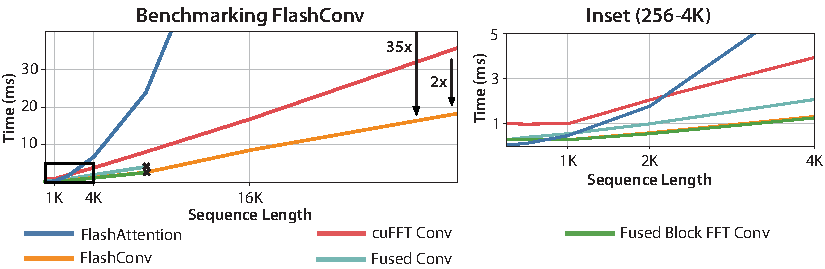
\includegraphics[width=\textwidth]{figs/benchmark_pdf.pdf}
    \caption{\label{fig:fftconv_speed}
      We compare the speed of different algorithms to perform FFT-based
      convolution, along with FlashAttention~\citep{dao2022flashattention} (the fastest attention
      implementation we know of).
      We use batch size 8, hidden dimension 1024, and varying sequence length
      from 256 to 32k, and measure on an A100-SMX4-40GB GPU.
      We see that kernel fusion gives up to 3.4$\times$ speedup over naive FFTConv
      for short sequences (up to 512), block FFT gives up to 2$\times$ speedup for
      medium length sequences (1k - 8k), and state-passing allows 2.3$\times$ faster
      FFTConv for long sequences (16k and above).
    }
\end{figure}